\section{Minimal number of 4-transpositions}

\paragraph{}
In this chapter we begin to apply Method~\ref{method} to prove that there are no sggis with some properties. The first applications are very easy. We only use the full method in Chapter~\ref{proof-5}.

\begin{lemma}
  \label{graphIsString}
  Let $\Gamma$ be a transitive sggi over $n$ points such that the permutation representation graph has exactly $n-1$ edges. Then the graph of $\Gamma$ is a chain.
\end{lemma}

\begin{proof}
  $\Gamma$ is transitive so its permutation representation graph is connected. Therefore, because there are $n-1$ edges for $n$ vertices, the graph must be a tree.

  \paragraph{}
  Suppose now that there is a vertex with at least three incident edges. These edges must be labeled with three different numbers $i, j, k$ that describe three different involutions, $\rho_i, \rho_j$ and $\rho_k$. But at least two of these involutions are not adjacent and so must commute. It will be considered that the involution $\rho_i$ and $\rho_k$ do not commute. By Property~\ref{intersection-patterns}, the permutation representation graph where only edges labeled with $i$ and $k$ are kept must only contain the patterns described in Property~\ref{intersection-patterns}.

  \paragraph{}
  On our case, there are already two edges labeled $i$ and $k$ that connect the same point to two different points. So the only way it can be extended to a good pattern is with an alternating square. But the graph cannot have an alternating square because it is a tree and thus does not contain any cycle.

  \paragraph{}
  Thus no vertex can have three edges but the graph must be connected, so the only solution is a string.
\end{proof}

\begin{lemma}
  \label{rho0atEnd2}
  Let $\Gamma$ be a sggi with generators $\rho_0, \rho_1 \dots$ such that its permutation representation graph is a string. If $\rho_0$ and $\rho_1$ are 2-transpositions, then an edge of $\rho_0$ must be placed at an end of the permutation representation graph.
\end{lemma}

\begin{proof}
  The proof of this is the same as the proof of Lemma~\ref{rho0atEnd}.
\end{proof}

\begin{lemma}
  \label{min-4-trans}
  Let $\Gamma$ be a sggi generating $A_{11}$. Then $\Gamma$ contains at least two 4-transpositions if it is of rank 4 and at least one 4-transposition if its rank is 5.
\end{lemma}

\begin{proof}
  Suppose that there exists a sggi of rank 5 with only 2-transpositions or a sggi of rank 4 with at most one 4-transposition. In both cases, there are at most 10 edges for 11 vertices. Lemma~\ref{graphIsString} can be applied and thus the permutation representation graph of $\Gamma$ is a string.

  \paragraph{Rank 5}
  In this case, there are five involutions and all of them are 2-transpositions. Thus, by Lemma~\ref{rho0atEnd}, a $\rho_0$ edge must be at one end of the graph. By duality, the same can be done with $\rho_4$ and so there is a $\rho_4$ edge at the other end.

  \paragraph{}
  Because the other end is occupied, the other edge of $\rho_0$ cannot go there. So a $\rho_1$ edge must be between the two $\rho_0$ edges (see the proof of Lemma~\ref{rho0atEnd2} for details). The same reasoning can be applied to $\rho_3$ by duality. At this point, the graph is the following:

  \begin{figure}[H]
    \begin{center}
      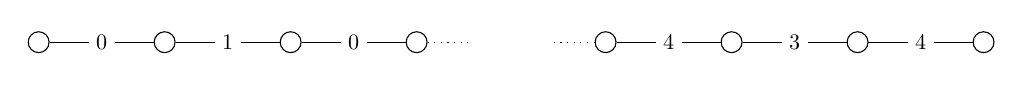
\begin{tikzpicture}[scale=.8]

        \begin{scope}[every node/.style={circle,draw, transform shape}]
          \node (1)  at (0,0)  {};
          \node (2)  at (2,0)  {};
          \node (3)  at (4,0)  {};
          \node (4)  at (6,0)  {};
          \node (8)  at (9,0)  {};
          \node (9)  at (11,0) {};
          \node (10) at (13,0) {};
          \node (11) at (15,0) {};
        \end{scope}

        \node (4b) at (7,0) {};
        \node (8b) at (8,0) {};

        \begin{scope}[every node/.style={fill=white, transform shape}]
          \begin{scope}[every edge/.style={draw}]
            \path (1)  edge node {$0$} (2);
            \path (2)  edge node {$1$} (3);
            \path (3)  edge node {$0$} (4);
            \path (4)  edge[style={dotted}] (4b);
            \path (8)  edge[style={dotted}] (8b);
            \path (8)  edge node {$4$} (9);
            \path (9)  edge node {$3$} (10);
            \path (10) edge node {$4$} (11);
          \end{scope}
        \end{scope}



      \end{tikzpicture}
      \caption{}
    \end{center}
  \end{figure}

  \paragraph{}
  The $\rho_0$ and $\rho_4$ edges must be connected to something but the only possibility is to use a $\rho_1$ and a $\rho_3$ edge. Now the graph is the following and two $\rho_2$ edges must still be added to it. But they would be adjacent to each other and that is forbidden in a permutation representation graph.

  \begin{figure}[H]
    \begin{center}
      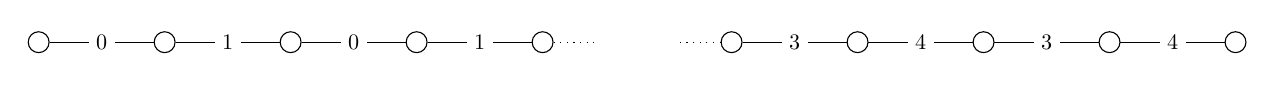
\begin{tikzpicture}[scale=.8]

        \begin{scope}[every node/.style={circle,draw, transform shape}]
          \node (1)  at (0,0)  {};
          \node (2)  at (2,0)  {};
          \node (3)  at (4,0)  {};
          \node (4)  at (6,0)  {};
          \node (5)  at (8,0)  {};
          \node (7)  at (11,0) {};
          \node (8)  at (13,0) {};
          \node (9)  at (15,0) {};
          \node (10) at (17,0) {};
          \node (11) at (19,0) {};
        \end{scope}

        \node (5b) at (9,0) {};
        \node (7b) at (10,0) {};

        \begin{scope}[every node/.style={fill=white, transform shape}]

          \begin{scope}[every edge/.style={draw}]
            \path (1)  edge node {$0$} (2);
            \path (2)  edge node {$1$} (3);
            \path (3)  edge node {$0$} (4);
            \path (4)  edge node {$1$} (5);
            \path (5)  edge[style={dotted}] (5b);
            \path (7)  edge[style={dotted}] (7b);
            \path (7)  edge node {$3$} (8);
            \path (8)  edge node {$4$} (9);
            \path (9)  edge node {$3$} (10);
            \path (10) edge node {$4$} (11);
          \end{scope}
        \end{scope}



      \end{tikzpicture}
      \caption{}
    \end{center}
  \end{figure}


  \paragraph{Rank 4}
  Since $A_{11}$ is transitive, there must be a 4-transposition. Now we prove that there must be at least two of them. To achieve this, we suppose that there is only one. By duality, there are two cases: either $\rho_0$ or $\rho_1$ is a 4-transposition. If $\rho_0$ is a 4-transposition, then $\rho_1$ is a 2-transposition but all $\rho_0$ must be surrounded by $\rho_1$ involutions which is impossible.

  \paragraph{}
  Suppose that $\rho_1$ is be a 4-transposition. Therefore $\rho_2$ and $\rho_3$ are 2-transpositions. By Lemma~\ref{rho0atEnd2}, a $\rho_3$ edge must be placed at an end, followed by a $\rho_2$ edge. For the other $\rho_3$ edge, there are two possibilities, it can be placed next to the first one or at the other end.

  \paragraph{}
  In the first case, the graph is the following. The only way it can be completed is by using a sequence $\rho_1, \rho_0, \rho_1, \rho_0, \rho_1$ but there is still a $\rho_1$ edge that cannot be placed.

  \begin{figure}[H]
    \begin{center}
      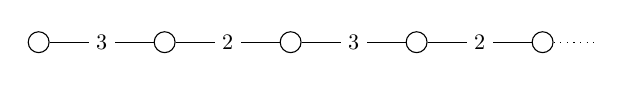
\begin{tikzpicture}[scale=.8]

        \begin{scope}[every node/.style={circle,draw, transform shape}]
          \node (1)  at (0,0)  {};
          \node (2)  at (2,0)  {};
          \node (3)  at (4,0)  {};
          \node (4)  at (6,0)  {};
          \node (5)  at (8,0)  {};
        \end{scope}

        \node (6)  at (9,0) {};

        \begin{scope}[every node/.style={fill=white, transform shape}]

          \begin{scope}[every edge/.style={draw}]
            \path (1)  edge node {$3$} (2);
            \path (2)  edge node {$2$} (3);
            \path (3)  edge node {$3$} (4);
            \path (4)  edge node {$2$} (5);
            \path (5)  edge[style={dotted}] (6);
          \end{scope}
        \end{scope}

      \end{tikzpicture}
      \caption{}
    \end{center}
  \end{figure}

\paragraph{}
For the second case, the graph is display in Figure~\ref{props-5-2}. On each side, it must be continued with a sequence $\rho_1, \rho_0, \rho_1$. Every edge would be used but the middle point would be linked with two $\rho_1$ edges and that is forbidden by Proposition~\ref{fixed-only-1}.

\begin{figure}[H]
  \begin{center}
    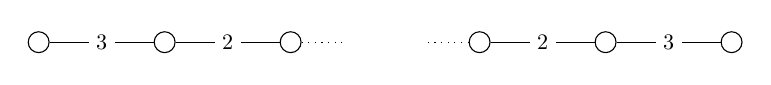
\begin{tikzpicture}[scale=.8]

      \begin{scope}[every node/.style={circle,draw, transform shape}]
        \node (1)  at (0,0)  {};
        \node (2)  at (2,0)  {};
        \node (3)  at (4,0)  {};
        \node (9)  at (7,0)  {};
        \node (10) at (9,0)  {};
        \node (11) at (11,0) {};
      \end{scope}

      \node (3b) at (5,0)  {};
      \node (9b) at (6,0)  {};


      \begin{scope}[every node/.style={fill=white, transform shape}]

        \begin{scope}[every edge/.style={draw}]
          \path (1)  edge node {$3$} (2);
          \path (2)  edge node {$2$} (3);
          \path (3)  edge[style={dotted}] (3b);
          \path (9)  edge[style={dotted}] (9b);
          \path (9)  edge node {$2$} (10);
          \path (10) edge node {$3$} (11);
        \end{scope}
      \end{scope}

    \end{tikzpicture}
    \caption{}
    \label{props-5-2}
  \end{center}
\end{figure}

\end{proof}

\section{Properties for $A_{11}$}

\begin{lemma}
  \label{no-simple-cycle}
  A string C-group representation graph of $A_{11}$ does not contains any simple cycle.
\end{lemma}

\begin{proof}
  In Propositions~\ref{rotation-pattern} and~\ref{linear-pattern}, we found two special cycles. We must now proof that those cycle cannot be connected a single and and cannot be extended to 11 points. This proof is easy but a quite long and not very interesting and is left to the reader.
\end{proof}

\begin{proposition}
  \label{adjacent-must-not-commute}
  If two consecutive generators commute then the generated group cannot be almost simple.
\end{proposition}

\begin{proof}
  If two consecutive $\rho_i$ and $\rho_{i+1}$ generators commute, then all generators $\le i$ commute with all generators $\ge i+1$ and thus the group can be written as a direct product. But it cannot be an almost simple group.
\end{proof}

\paragraph{}
Due to Lemmas~\ref{continue-alternating-square}, \ref{square-connection} and~\ref{continue-double-edge}, we know that double edges or alternating square with non consecutive indices can lead to a long sequence of alternating squares. Now we prove that in the case of a rank 5 sggi, no $\rho_0$ and $\rho_4$ edges can be adjacent.

\begin{lemma}
  \label{lemma-forbidden-alternating-square}
  Let $\Gamma$ be a sggi generating $A_{11}$ of rank 5. Then its permutation representation graph does not contain an alternating square between $\rho_0$ and $\rho_4$.
\end{lemma}

\begin{proof}
  In this graph we apply Method~\ref{method}. First we must choose a starting pattern, it is very easy here: it will be an alternating square $[\rho_0, \rho_4]$. The second step of the method is to try to build a connected graph with only even involutions. If no graph is found, that means that the pattern chosen is impossible.

  \paragraph{}
  We start with an alteranting square between $\rho_0$ and $\rho_4$.

  \begin{figure}[H]
    \begin{center}
      \begin{tikzpicture}[scale=.8]

        \begin{scope}[every node/.style={circle,draw, transform shape}]
          \node (1)  at (0,2)  {};
          \node (2)  at (0,0)  {};
          \node (3)  at (2,2)  {};
          \node (4)  at (2,0)  {};
          \node (5)  at (4,0)  {};
          \node (6)  at (6,0)  {};
          \node (7)  at (8,0)  {};
          \node (8)  at (10,0) {};
          \node (9)  at (12,0) {};
          \node (10) at (14,0) {};
          \node (11) at (16,0) {};
        \end{scope}

        \begin{scope}[every node/.style={fill=white, transform shape}]

          \begin{scope}[every edge/.style={draw}]
            \path (1)  edge node {$0$} (2);
            \path (3)  edge node {$0$} (4);
            \path (1)  edge node {$4$} (3);
            \path (2)  edge node {$4$} (4);
          \end{scope}
        \end{scope}

      \end{tikzpicture}
      \caption{}
    \end{center}
  \end{figure}

  \paragraph{}
  By Lemma~\ref{continue-alternating-square}, we need to find one sequence of alternating squares until the difference between indices is two. At this point the sequence can be connected by a single edge. Therefore this sequence contains at least 3 squares.

  \paragraph{}
  From the square $[\rho_0, \rho_4]$, we can place an adjacent square $[\rho_1, \rho_4]$ or $[\rho_0, \rho_3]$. But those solutions are dual, thus we only consider the last one.

  \begin{figure}[H]
    \begin{center}
      \begin{tikzpicture}[scale=.8]

        \begin{scope}[every node/.style={circle,draw, transform shape}]
          \node (1)  at (0,2)  {};
          \node (2)  at (0,0)  {};
          \node (3)  at (2,2)  {};
          \node (4)  at (2,0)  {};
          \node (5)  at (4,2)  {};
          \node (6)  at (4,0)  {};
          \node (7)  at (6,0)  {};
          \node (8)  at (8,0) {};
          \node (9)  at (10,0) {};
          \node (10) at (12,0) {};
          \node (11) at (14,0) {};
        \end{scope}

        \begin{scope}[every node/.style={fill=white, transform shape}]

          \begin{scope}[every edge/.style={draw}]
            \path (1)  edge node {$0$} (2);
            \path (3)  edge node {$0$} (4);
            \path (5)  edge node {$0$} (6);
            \path (3)  edge node {$3$} (5);
            \path (4)  edge node {$3$} (6);
            \path (1)  edge node {$4$} (3);
            \path (2)  edge node {$4$} (4);
          \end{scope}
        \end{scope}

      \end{tikzpicture}
      \caption{}
    \end{center}
  \end{figure}

  \paragraph{}
  Now, the rotation pattern seen in Proposition~\ref{rotation-pattern} cannot be placed because the difference between the indices of the square $[\rho_1, \rho_4]$ is not 2. Thus the next square must be a $[\rho_0, \rho_2]$ or a $[\rho_0, \rho_4]$. If we use the last case, we are stuck because all 4 $\rho_0$ edges have been used and none of the square of the sequence have a difference between their indices of 2. Thus the sequence of alternating squares cannot be connected by an alternating square nor a double edge nor a simple edge. So the next square must be $[\rho_0, \rho_2]$.

  \begin{figure}[H]
    \begin{center}
      \begin{tikzpicture}[scale=.8]

        \begin{scope}[every node/.style={circle,draw, transform shape}]
          \node (1)  at (0,2)  {};
          \node (2)  at (0,0)  {};
          \node (3)  at (2,2)  {};
          \node (4)  at (2,0)  {};
          \node (5)  at (4,2)  {};
          \node (6)  at (4,0)  {};
          \node (7)  at (6,2)  {};
          \node (8)  at (6,0)  {};
          \node (9)  at (8,0)  {};
          \node (10) at (10,0) {};
          \node (11) at (12,0) {};
        \end{scope}

        \begin{scope}[every node/.style={fill=white, transform shape}]

          \begin{scope}[every edge/.style={draw}]
            \path (1)  edge node {$0$} (2);
            \path (3)  edge node {$0$} (4);
            \path (5)  edge node {$0$} (6);
            \path (7)  edge node {$0$} (8);
            \path (5)  edge node {$2$} (7);
            \path (6)  edge node {$2$} (8);
            \path (3)  edge node {$3$} (5);
            \path (4)  edge node {$3$} (6);
            \path (1)  edge node {$4$} (3);
            \path (2)  edge node {$4$} (4);
          \end{scope}
        \end{scope}

      \end{tikzpicture}
      \caption{}
    \end{center}
  \end{figure}

  \paragraph{}
  The sequence cannot be continued because there are no more $\rho_0$ edge. Moreover none of the patterns seen in Proposition~\ref{rotation-pattern} and~\ref{linear-pattern} can be placed for the same reason. The square $[\rho_0, \rho_2]$ must thus be adjacent to a single $\rho_1$ edge by Lemma~\ref{square-connection}

  \begin{figure}[H]
    \begin{center}
      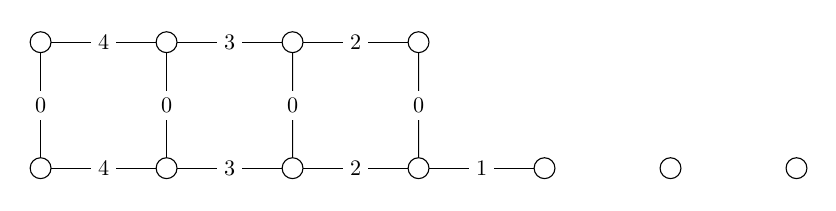
\begin{tikzpicture}[scale=.8]

        \begin{scope}[every node/.style={circle,draw, transform shape}]
          \node (1)  at (0,2)  {};
          \node (2)  at (0,0)  {};
          \node (3)  at (2,2)  {};
          \node (4)  at (2,0)  {};
          \node (5)  at (4,2)  {};
          \node (6)  at (4,0)  {};
          \node (7)  at (6,2)  {};
          \node (8)  at (6,0)  {};
          \node (9)  at (8,0)  {};
          \node (10) at (10,0) {};
          \node (11) at (12,0) {};
        \end{scope}

        \begin{scope}[every node/.style={fill=white, transform shape}]

          \begin{scope}[every edge/.style={draw}]
            \path (1)  edge node {$0$} (2);
            \path (3)  edge node {$0$} (4);
            \path (5)  edge node {$0$} (6);
            \path (7)  edge node {$0$} (8);
            \path (8)  edge node {$1$} (9);
            \path (5)  edge node {$2$} (7);
            \path (6)  edge node {$2$} (8);
            \path (3)  edge node {$3$} (5);
            \path (4)  edge node {$3$} (6);
            \path (1)  edge node {$4$} (3);
            \path (2)  edge node {$4$} (4);
          \end{scope}
        \end{scope}

      \end{tikzpicture}
      \caption{}
    \end{center}
  \end{figure}

  \paragraph{}
  To link the two remaining points, we only need two edges but the total amount of edges would be odd and that is forbidden because we want that the generated group to be $A_{11}$. To restore parity we need to create a double edge or an alternating square. The number of points is insufficient to create an alternating square, so we must create a double edge and the difference between its indices must be two. All $\rho_0$ edges have already been used, so the possibilities for double edges are $(\rho_1, \rho_3)$ and $(\rho_2, \rho_4)$ but then the number of $\rho_3$ and $\rho_4$ edges becomes odd. So it is impossible to connect all points if $\rho_0$ is a 4-transposition and there is an alternating square between $\rho_0$ and $\rho_4$.

  \paragraph{}
  Thus there are no permutation representation graphs of $A_{11}$ that contain an alternating square $[\rho_0, \rho_4]$.
\end{proof}

\begin{lemma}
  \label{lemma-forbidden-double-edge}
  In a permutation representation graph of rank 5 with 11 points, it is impossible to have a double edge between $\rho_0$ and $\rho_4$.
\end{lemma}

\begin{proof}
  By Lemma~\ref{continue-double-edge}, to extend a double edge $(\rho_0, \rho_4)$, we must use an alternating square. We have two possibilities, either $[\rho_0, \rho_3]$ or $[\rho_1, \rho_4]$. Those two solutions are dual, so we only study the first one. Another edge must be added in order to be connected to single edge by Proposition~\ref{square-connection}. The pattern seen in Proposition~\ref{rotation-pattern} cannot be applied because the difference between the indices is not 2, thus we must stay linear and the graph must be $[\rho_0, \rho_2]$. We have the following graph:

  \begin{figure}[H]
    \begin{center}
      \begin{tikzpicture}[scale=.8]

        \begin{scope}[every node/.style={circle,draw, transform shape}]
          \node (1)  at (0,2)  {};
          \node (2)  at (0,0)  {};
          \node (3)  at (2,2)  {};
          \node (4)  at (2,0)  {};
          \node (5)  at (4,2)  {};
          \node (6)  at (4,0)  {};
          \node (7)  at (6,0)  {};
          \node (8)  at (8,0)  {};
          \node (9)  at (10,0) {};
          \node (10) at (12,0) {};
          \node (11) at (14,0) {};
        \end{scope}

        \begin{scope}[every node/.style={fill=white, transform shape}]

          \begin{scope}[every edge/.style={draw}]
            \path (1)  edge[bend right=30] node {$0$} (2);
            \path (3)  edge node {$0$} (4);
            \path (5)  edge node {$0$} (6);
            \path (3)  edge node {$2$} (5);
            \path (4)  edge node {$2$} (6);
            \path (1)  edge node {$3$} (3);
            \path (2)  edge node {$3$} (4);
            \path (1)  edge[bend left=30] node {$4$} (2);
          \end{scope}
        \end{scope}

      \end{tikzpicture}
      \caption{}
    \end{center}
  \end{figure}

  \paragraph{}
  In order to be able to link a single edge to this component, we must end the sequence here or add two extra squares. But a rotation pattern must be used because there are only 4 $\rho_0$ edges. If the rotation pattern is added, the graph is the following one:

  \begin{figure}[H]
    \begin{center}
      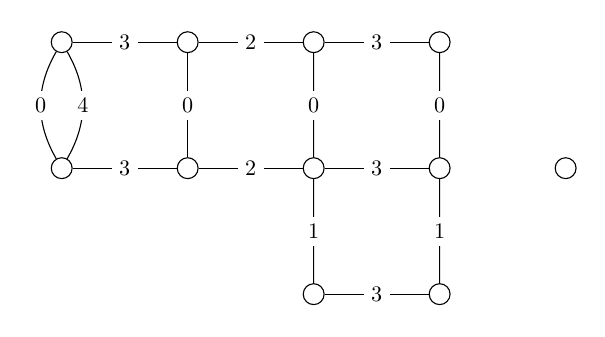
\begin{tikzpicture}[scale=.8]

        \begin{scope}[every node/.style={circle,draw, transform shape}]
          \node (1)  at (0,2)  {};
          \node (2)  at (0,0)  {};
          \node (3)  at (2,2)  {};
          \node (4)  at (2,0)  {};
          \node (5)  at (4,2)  {};
          \node (6)  at (4,0)  {};
          \node (7)  at (6,2)  {};
          \node (8)  at (6,0)  {};
          \node (9)  at (4,-2)  {};
          \node (10) at (6,-2)  {};
          \node (11) at (8,0) {};
        \end{scope}

        \begin{scope}[every node/.style={fill=white, transform shape}]

          \begin{scope}[every edge/.style={draw}]
            \path (1)  edge[bend right=30] node {$0$} (2);
            \path (3)  edge node {$0$} (4);
            \path (5)  edge node {$0$} (6);
            \path (7)  edge node {$0$} (8);
            \path (6)  edge node {$1$} (9);
            \path (8)  edge node {$1$} (10);
            \path (3)  edge node {$2$} (5);
            \path (4)  edge node {$2$} (6);
            \path (1)  edge node {$3$} (3);
            \path (2)  edge node {$3$} (4);
            \path (5)  edge node {$3$} (7);
            \path (6)  edge node {$3$} (8);
            \path (9)  edge node {$3$} (10);
            \path (1)  edge[bend left=30] node {$4$} (2);
          \end{scope}
        \end{scope}

      \end{tikzpicture}
      \caption{}
    \end{center}
  \end{figure}

  \paragraph{}
  We used 5 $\rho_3$  edges and there are only 4 of them. Thus the sequence of alternating squares must not be extended beyond length 2. Thus it must be connected by a single edge.

  \begin{figure}[H]
    \begin{center}
      \begin{tikzpicture}[scale=.8]

        \begin{scope}[every node/.style={circle,draw, transform shape}]
          \node (1)  at (0,2)  {};
          \node (2)  at (0,0)  {};
          \node (3)  at (2,2)  {};
          \node (4)  at (2,0)  {};
          \node (5)  at (4,2)  {};
          \node (6)  at (4,0)  {};
          \node (7)  at (6,0)  {};
          \node (8)  at (8,0)  {};
          \node (9)  at (10,0) {};
          \node (10) at (12,0) {};
          \node (11) at (14,0) {};
        \end{scope}

        \begin{scope}[every node/.style={fill=white, transform shape}]

          \begin{scope}[every edge/.style={draw}]
            \path (1)  edge[bend right=30] node {$0$} (2);
            \path (3)  edge node {$0$} (4);
            \path (5)  edge node {$0$} (6);
            \path (6)  edge node {$1$} (7);
            \path (3)  edge node {$2$} (5);
            \path (4)  edge node {$2$} (6);
            \path (1)  edge node {$3$} (3);
            \path (2)  edge node {$3$} (4);
            \path (1)  edge[bend left=30] node {$4$} (2);
          \end{scope}
        \end{scope}

      \end{tikzpicture}
      \caption{}
    \end{center}
  \end{figure}

  \paragraph{}
  We have two issues in this graph: there is only one $\rho_4$ edge and if we link all remaining points with single edge, the total number of edges would be odd.

  \paragraph{}
  The $\rho_4$ edge cannot be placed on the existing component. So it must be placed between two fixed points. Thus we need to link this edge to the rest of the graph, and because we have only two points remaining, it must be done using a $\rho_2$ and $\rho_3$ edges. For now, we have the following graph:


  \begin{figure}[H]
    \begin{center}
      \begin{tikzpicture}[scale=.8]

        \begin{scope}[every node/.style={circle,draw, transform shape}]
          \node (1)  at (0,2)  {};
          \node (2)  at (0,0)  {};
          \node (3)  at (2,2)  {};
          \node (4)  at (2,0)  {};
          \node (5)  at (4,2)  {};
          \node (6)  at (4,0)  {};
          \node (7)  at (6,0)  {};
          \node (8)  at (8,0)  {};
          \node (9)  at (12,0) {};
          \node (10) at (10,0) {};
          \node (11) at (14,0) {};
        \end{scope}

        \begin{scope}[every node/.style={fill=white, transform shape}]

          \begin{scope}[every edge/.style={draw}]
            \path (1)  edge[bend right=30] node {$0$} (2);
            \path (3)  edge node {$0$} (4);
            \path (5)  edge node {$0$} (6);
            \path (6)  edge node {$1$} (7);
            \path (3)  edge node {$2$} (5);
            \path (4)  edge node {$2$} (6);
            \path (7)  edge node {$2$} (8);
            \path (1)  edge node {$3$} (3);
            \path (2)  edge node {$3$} (4);
            \path (8)  edge node {$3$} (10);
            \path (1)  edge[bend left=30] node {$4$} (2);
            \path (9)  edge node {$4$} (10);
          \end{scope}
        \end{scope}

      \end{tikzpicture}
      \caption{}
    \end{center}
  \end{figure}

  \paragraph{}
  The number of $\rho_0$ edges is still odd and there is room for an additional one. Thus the graph cannot be turned into the permutation representation graph of a sggi of rank 5 of $A_{11}$.


\end{proof}

\begin{corollary}
  \label{0-4-no-share}
  In a permutation representation graph of $A_{11}$ of rank 5, no $\rho_0$ edges can be adjacent to a $\rho_4$ edge.
\end{corollary}
